\section{给定端点的最短路径}
\label{sec:riem-shortest-paths}

上一节固定的是起点和初始速度，本节固定的是两个端点。问题变成：在所有连接$p$与$q$的分段光滑曲线中，长度能否达到内在距离$d_g(p,q)$，达到时曲线是什么样子。我们分三步回答。先比较长度与能量，说明长度最短且匀速的曲线满足测地线方程；再证明足够短的测地线确实最短；最后陈述保证最短曲线存在的整体条件。每一步的结论都比前一步的要求多，不能互相替代。

\subsection{长度与能量的变分}
\label{sec:riem-length-energy-variation}

长度的被积函数$\lVert\dot\gamma\rVert_g$含有平方根，直接求导不便，而且长度对任何单调换参数都不变，同一条路线有无穷多种参数化都是“最优”的。常用的办法是改用能量。对$\gamma:[a,b]\to M$，定义\term{曲线能量}（energy of a curve）
\begin{equation}
E(\gamma)=\frac12\int_a^b\lVert\dot\gamma(t)\rVert_g^2\,\mathrm dt .
\label{eq:riem-energy}
\end{equation}

\paragraph{长度与能量的比较}
由Cauchy--Schwarz不等式，把$\lVert\dot\gamma\rVert_g$看成与常函数$1$作内积：
\[
L_g(\gamma)^2=\Bigl(\int_a^b1\cdot\lVert\dot\gamma\rVert_g\,\mathrm dt\Bigr)^2\leq(b-a)\int_a^b\lVert\dot\gamma\rVert_g^2\,\mathrm dt .
\]
右端等于$2(b-a)E(\gamma)$，所以
\begin{equation}
L_g(\gamma)^2\leq2(b-a)E(\gamma),
\label{eq:riem-length-energy}
\end{equation}
等号成立当且仅当$\lVert\dot\gamma\rVert_g$在$[a,b]$上几乎处处为常数，即曲线匀速。

因此在固定时间区间上，走同一条路线时忽快忽慢只会增加能量。例如在实数轴上走$[0,1]$这段路线，$x(t)=t^2$，$t\in[0,1]$，长度$L=1$，能量却是
\[
E=\frac12\int_0^1(2t)^2\,\mathrm dt=\frac23 .
\]
匀速的$x(t)=t$给出$E=\tfrac12=L^2/2$，式~\eqref{eq:riem-length-energy}取等号。能量最小的曲线必然匀速。速度处处非零的曲线可以重新参数化为匀速，所以在匀速曲线之间比较能量，等同于比较长度。

\paragraph{能量的驻定条件}
现在考察端点固定的扰动。设$\gamma$落在一张坐标图内，坐标为$x(t)$；取光滑的$h:[a,b]\to\mathbb R^n$，$h(a)=h(b)=0$，对足够小的$\varepsilon$令$x_\varepsilon=x+\varepsilon h$。若对所有这样的$h$都有
\[
\frac{\mathrm d}{\mathrm d\varepsilon}E(\gamma_\varepsilon)\Big|_{\varepsilon=0}=0,
\]
就称$\gamma$是能量的驻定曲线。

能量的被积函数是
\[
\mathscr L(x,\dot x)=\frac12\sum_{i,j}g_{i,j}(x)\,\dot x_i\dot x_j .
\]
对这类积分，所用的结论是Euler--Lagrange关系：若$\mathscr L$光滑，$x$为$C^2$曲线，则$x$在端点固定的扰动下驻定当且仅当
\begin{equation}
\frac{\partial\mathscr L}{\partial x_k}-\frac{\mathrm d}{\mathrm dt}\frac{\partial\mathscr L}{\partial\dot x_k}=0,\qquad k=1,\ldots,n .
\label{eq:riem-euler-lagrange}
\end{equation}
它的推导是对$\varepsilon$求导后分部积分，边界项因$h(a)=h(b)=0$消失，再由$h$的任意性得到被积系数为零；一般泛函的变分理论可参考\BookChapterRef{chap:functional-optimization-variation}{卷五“泛函优化与变分”章}。

把能量代入。对$x_k$和$\dot x_k$分别求偏导，
\[
\frac{\partial\mathscr L}{\partial x_k}=\frac12\sum_{i,j}\partial_kg_{i,j}\,\dot x_i\dot x_j,\qquad
\frac{\partial\mathscr L}{\partial\dot x_k}=\sum_jg_{k,j}\dot x_j .
\]

后一式对时间求导，用链式法则：
\[
\frac{\mathrm d}{\mathrm dt}\sum_jg_{k,j}\dot x_j=\sum_jg_{k,j}\ddot x_j+\sum_{i,j}\partial_ig_{k,j}\,\dot x_i\dot x_j .
\]
第二项对$i,j$对称化，写成$\frac12\sum_{i,j}(\partial_ig_{k,j}+\partial_jg_{k,i})\dot x_i\dot x_j$。

代回式~\eqref{eq:riem-euler-lagrange}并取负号，得到
\[
\sum_jg_{k,j}\ddot x_j+\frac12\sum_{i,j}\bigl(\partial_ig_{k,j}+\partial_jg_{k,i}-\partial_kg_{i,j}\bigr)\dot x_i\dot x_j=0 .
\]
括号恰是式~\eqref{eq:riem-christoffel}中的组合。两边乘$\bm G^{-1}$，得到测地线方程~\eqref{eq:riem-geodesic-equation}。曲线跨越多张图时，用支撑在单张图内的扰动逐段推导，结论相同。

单位球面可以这样快速验算。被积函数是
\[
\mathscr L=\tfrac12\bigl(\dot\theta^2+\sin^2\theta\,\dot\phi^2\bigr).
\]

对$\theta$和对$\phi$的方程分别是
\[
\ddot\theta-\sin\theta\cos\theta\,\dot\phi^2=0,\qquad
\frac{\mathrm d}{\mathrm dt}\bigl(\sin^2\theta\,\dot\phi\bigr)=0 .
\]
第二式展开后就是例~\ref{ex:riem-geodesic-examples}中的第二个方程。

这样得到两条结论。光滑曲线是能量的驻定曲线，当且仅当它是测地线。若匀速曲线在所有连接相同端点的曲线中长度最短，则它也是能量最小的，因而是测地线。长度本身的驻定曲线则只确定路线、不确定参数化：长度的Euler--Lagrange方程对任意换参数都成立，换成匀速参数后才是测地线方程。

\paragraph{驻定不等于最短}
驻定条件只是一阶条件，类似卷一中导数为零的点不一定是最小值点。完整单位圆上，从$(1,0)$到$(0,-1)$，顺时针的短弧长$\pi/2$，逆时针的长弧长$3\pi/2$，二者匀速参数化后都是测地线，只有前者最短。单位球面上沿大圆从$p$出发走过对跖点再继续，同样是测地线，却比反方向的另一段大圆弧长。驻定曲线是否最短，还要额外比较。

\subsection{局部最短性}
\label{sec:riem-local-minimality}

上面的反例都发生在曲线较长时。下面证明：足够短的测地线一定最短。论证用到正常邻域中径向与“横向”方向的正交关系。平面上，同心圆与半径处处垂直；下面的Gauss引理说明，在指数映射的图像里同样如此。

\begin{lemma}[Gauss引理]
\label{lem:riem-gauss-lemma}
设$\exp_p$在$T_pM$中以$\bm 0$为心、半径$\varepsilon$的球$B_\varepsilon(\bm 0)$上是微分同胚。对$\bm v\in B_\varepsilon(\bm 0)$，$\bm v\neq\bm 0$，以及任意$\bm w\in T_pM$，有
\begin{equation}
g\bigl(\mathrm d(\exp_p)_{\bm v}(\bm v),\,\mathrm d(\exp_p)_{\bm v}(\bm w)\bigr)=g_p(\bm v,\bm w).
\label{eq:riem-gauss-lemma}
\end{equation}
特别地，径向测地线的速度与由长度等于$\lVert\bm v\rVert_g$的切向量在$\exp_p$下的像组成的球面在交点处正交。
\end{lemma}

\begin{proof}
构造一族从$p$出发的测地线：对$t\in[0,1]$和足够小的$s$，令
\[
f(t,s)=\exp_p\bigl(t(\bm v+s\bm w)\bigr).
\]
$f$是光滑的，固定$s$时它是初速度为$\bm v+s\bm w$的测地线。记$T=\partial_tf$，$S=\partial_sf$，这是沿这族曲线的两个向量场。

我们需要两个事实。第一，$T$沿$t$方向的协变导数为零，这是测地线方程：$D_tT=0$。第二，$D_tS=D_sT$，这是无挠条件的结果。在坐标中，$D_tS$的$k$分量是
\[
\frac{\partial^2x_k}{\partial t\,\partial s}+\sum_{i,j}\Gamma^k_{i,j}\frac{\partial x_i}{\partial t}\frac{\partial x_j}{\partial s},
\]
由$\Gamma^k_{i,j}$的对称性，它关于$t,s$对称。

对$g(T,S)$关于$t$求导，用度量相容和上面两个事实：
\[
\partial_t\,g(T,S)=g(D_tT,S)+g(T,D_tS)=g(T,D_sT).
\]

右端等于$\tfrac12\partial_s\,g(T,T)$。测地线匀速，所以$g(T,T)$等于初速度的长度平方$\lVert\bm v+s\bm w\rVert_g^2$，与$t$无关。取$s=0$，得到
\[
\partial_t\,g(T,S)\big|_{s=0}=\tfrac12\frac{\mathrm d}{\mathrm ds}\lVert\bm v+s\bm w\rVert_g^2\Big|_{s=0}=g_p(\bm v,\bm w).
\]

右端是常数。在$t=0$处，$f(0,s)=p$与$s$无关，所以$S(0,0)=\bm 0$，$g(T,S)$从$0$开始。沿$t$积分到$t=1$，得到
\[
g(T,S)\big|_{(1,0)}=g_p(\bm v,\bm w).
\]
而$T(1,0)=\mathrm d(\exp_p)_{\bm v}(\bm v)$，$S(1,0)=\mathrm d(\exp_p)_{\bm v}(\bm w)$，这就是式~\eqref{eq:riem-gauss-lemma}。

取$\bm w$与$\bm v$垂直，右端为零，所以径向方向与测地球面垂直。
\end{proof}

称$\exp_p(B_\varepsilon(\bm 0))$为$p$的半径$\varepsilon$的测地球。Gauss引理把图~\ref{fig:riem-exp-map}(c)的分解变成了等式：速度分解成径向和横向两部分，二者互相垂直，勾股定理可以用。

\begin{theorem}[径向测地线的最短性]
\label{thm:riem-radial-minimizing}
设$\exp_p$在$B_\varepsilon(\bm 0)\subseteq T_pM$上是微分同胚，$q=\exp_p(\bm v)$，$\lVert\bm v\rVert_g<\varepsilon$。则径向测地线$\sigma(t)=\exp_p(t\bm v)$，$t\in[0,1]$，长度为$\lVert\bm v\rVert_g$，并且任何从$p$到$q$的分段光滑曲线长度都不小于$\lVert\bm v\rVert_g$。因此
\begin{equation}
d_g(p,q)=\lVert\bm v\rVert_g .
\label{eq:riem-radial-distance}
\end{equation}
\end{theorem}

\begin{proof}
$\sigma$是初速度为$\bm v$的测地线，匀速，所以$L_g(\sigma)=\lVert\bm v\rVert_g$。设$\gamma:[a,b]\to M$是任一从$p$到$q$的分段光滑曲线。可以假设$\gamma$在$t>a$时不再经过$p$，否则从最后一次经过$p$的时刻开始考虑，长度只会变小。

先设$\gamma$始终留在测地球中。对$t>a$写
\[
\gamma(t)=\exp_p\bigl(\rho(t)\bm u(t)\bigr),\qquad\rho(t)>0,\quad\lVert\bm u(t)\rVert_g=1 .
\]

由链式法则，
\[
\dot\gamma=\mathrm d(\exp_p)\bigl(\dot\rho\,\bm u+\rho\,\dot{\bm u}\bigr),
\]
其中$\dot{\bm u}\perp\bm u$，因为$\lVert\bm u\rVert_g$恒为$1$。在式~\eqref{eq:riem-gauss-lemma}中取$\bm v=\rho\bm u$、$\bm w=\bm u$，得到$\mathrm d(\exp_p)(\bm u)$的长度为$1$。再取$\bm w=\rho\dot{\bm u}$，得到它与$\mathrm d(\exp_p)(\rho\dot{\bm u})$正交。

于是两部分互相垂直，由勾股定理，
\[
\lVert\dot\gamma\rVert_g^2=\dot\rho^2+\bigl\lVert\mathrm d(\exp_p)(\rho\dot{\bm u})\bigr\rVert_g^2\geq\dot\rho^2 .
\]

积分，并让积分下限趋于$a$（此时$\rho\to0$），得到
\[
L_g(\gamma)\geq\int_a^b\lvert\dot\rho\rvert\,\mathrm dt\geq\rho(b)-\lim_{t\to a^+}\rho(t)=\lVert\bm v\rVert_g .
\]

若$\gamma$离开测地球，它在离开前必须先到达每个半径$\delta<\varepsilon$的测地球面。对满足$\lVert\bm v\rVert_g<\delta<\varepsilon$的$\delta$，把上面的论证用于从$p$到第一次到达半径$\delta$球面的那一段，得到$L_g(\gamma)\geq\delta>\lVert\bm v\rVert_g$。两种情形合起来即得结论。
\end{proof}

证明中的不等式还给出等号条件：长度恰为$\lVert\bm v\rVert_g$的曲线必须$\rho$单调、横向分量为零，也就是沿径向走。所以测地球内$p$到$q$的最短曲线，除参数化外只有径向测地线这一条。

定理比较的是从中心$p$出发的所有曲线，包括离开测地球的曲线，所以结论是真正的距离等式。它对测地球中任意两点之间的连线并不直接给出结论：两点都不是中心时，需要更小的凸正常邻域，在那里任意两点由唯一一条留在邻域内的最短测地线连接。这一进一步的局部结论的证明较长，读者可查阅Lee的教材\scite{math-lee2018riemannian}。称长度等于两端点内在距离的测地线为\term{最短测地线}（minimizing geodesic）。

\paragraph{局部最短不意味着全局最短或唯一}
定理~\ref{thm:riem-radial-minimizing}给出：每条测地线的足够短的一段都是最短测地线。但整条测地线可以不是最短的。取半径为$1$的圆柱面$\{(x,y,z):x^2+y^2=1\}$，曲线$t\mapsto(\cos t,\sin t,ct)$匀速，环境加速度$(-\cos t,-\sin t,0)$沿法向，所以这些螺旋线是测地线。

考虑连接$p_0=(1,0,0)$与$p_1=(1,0,\pi)$的曲线。竖直线段长$\pi$。绕$k$圈的螺旋线$t\mapsto(\cos t,\sin t,\tfrac{t}{2k})$，$t\in[0,2\pi k]$，速率是$\sqrt{1+1/(4k^2)}$，长度为
\[
L_k=2\pi k\sqrt{1+\frac1{4k^2}}=\pi\sqrt{4k^2+1}.
\]
$k=1,2$时分别是$\pi\sqrt5\approx7.02$和$\pi\sqrt{17}\approx12.95$，反向绕圈的情形相同。连接同一对端点的测地线有无穷多条，局部都是最短的，只有竖直线段全局最短。

图~\ref{fig:riem-cylinder-geodesics}把这些曲线放到圆柱展开的平面上：$p_1$有无穷多个“复本”，每条测地线就是通向其中一个复本的直线段。球面的对跖点则说明，最短测地线本身也可以不唯一：所有从$p$到$-p$的半个大圆都是最短的。

\begin{BookInlineFigure}
  \centering
  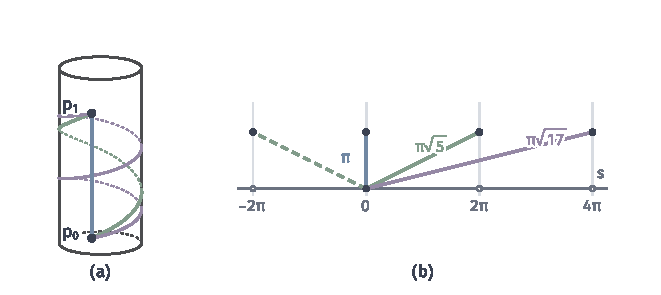
\includegraphics[width=112mm]{figures/04-spaces-measures-and-geometry/04-manifolds/matplotlib/riem-cylinder-geodesics/figure.pdf}
  \caption{圆柱面上连接同一对点的多条测地线。(a)单位圆柱上的$p_0=(1,0,0)$、$p_1=(1,0,\pi)$，蓝色竖直线段长$\pi$，绿色、紫色分别绕$1$圈、$2$圈。(b)沿圆周方向展开，竖线是$s=2\pi k$处$p_0$与$p_1$的复本，每条测地线是从原点到一个复本的线段，长度分别为$\pi$、$\pi\sqrt5$、$\pi\sqrt{17}$；虚线是反向绕圈的情形。}
  \label{fig:riem-cylinder-geodesics}
\end{BookInlineFigure}

\subsection{最短路径的存在}
\label{sec:riem-shortest-existence}

局部最短性只回答“短距离内测地线就是最短路”，不回答相距较远的两点之间是否有最短路。图~\ref{fig:riem-punctured-plane}的穿孔平面表明，答案可以是否定的：缺口使逼近下确界的曲线序列没有极限。排除这类缺口的条件是度量完备性。

\begin{theorem}[Hopf--Rinow定理]
\label{thm:riem-hopf-rinow}
设$(M,g)$是有限维、连通、无边界的黎曼流形。下列条件等价：
\begin{enumerate}
\item 度量空间$(M,d_g)$完备；
\item $M$是\term{测地完备}（geodesically complete）的，即每条测地线都能延拓到全体实数时间；
\item 存在某一点$p$，使$\exp_p$在整个$T_pM$上有定义；
\item $M$中有界闭集都是紧集。
\end{enumerate}
满足这些条件时，任意两点$p,q\in M$之间存在长度为$d_g(p,q)$的最短测地线。
\end{theorem}

这一定理称为\term{Hopf--Rinow定理}（Hopf--Rinow theorem）。证明需要依次比较几种完备性，篇幅较长，读者可查阅前引教材。它的机制可以这样理解：条件(3)使从$p$出发的每个方向都能一直走下去。对远处的点$q$，在$p$附近的测地球面上取与$q$距离最小的点，沿指向它的方向走测地线，可以证明这条测地线一直“对准”$q$，走过距离$d_g(p,q)$时恰好到达$q$。完备性保证这一过程不会中途掉进缺口。

\paragraph{条件的作用}
紧的无边界黎曼流形总是完备的：紧度量空间中的Cauchy列有收敛子列，从而本身收敛（第~\ref{chap:metric-spaces}章）。所以球面、环面等闭曲面上任意两点之间都有最短测地线。穿孔平面与开单位球不完备：前者中趋于原点的点列是Cauchy列却不收敛，后者中直线测地线在有限时间到达缺失的边界。

定理的最后结论只是充分条件。开单位球不完备，但它是凸集，任意两点之间的线段留在球内，是最短测地线；穿孔平面则连这一点也做不到。所以“任意两点都有最短路”不能反推完备性，而缺少完备性时，最短路是否存在要具体判断。

\paragraph{存在与唯一}
Hopf--Rinow定理保证存在，不保证唯一。球面对跖点之间有无穷多条最短测地线，圆柱面上位于同一水平圆的对径点之间有两条。存在性也不能由测地线方程的局部存在唯一性推出：后者固定的是初始速度，回答的是“从这个方向出发会走到哪里”；端点问题要找的是“哪个初始速度能恰好到达$q$且最短”，这需要比较全部路线，依赖流形的整体结构。
